%%%%%%%%%%%%%%%%%%%%%%%%%%%%%%%%%%%%%%%%%%%%%%%%%%
\section{Quantum software architecture}
% classical structure
Computer languages are influenced by the structure of the computer. In classical computers, languages developed historically in order to increase abstraction and ease the task of the programmer. To begin with, assembly language replaced machine code because it is easier to remember a mnemonic like ADD rather than a string of ones and zeros representing the same thing. The C programming language was invented to make common programming constructions such as if-statements and while-loops easier to program, using machine independent syntax. C is a compiled language, meaning that it needs to be converted into machine code before it can run. There is a different compiler for each computer architecture, which converts C into the specific instructions that can be executed on that machine. 

\begin{figure}[H]
    \centering
    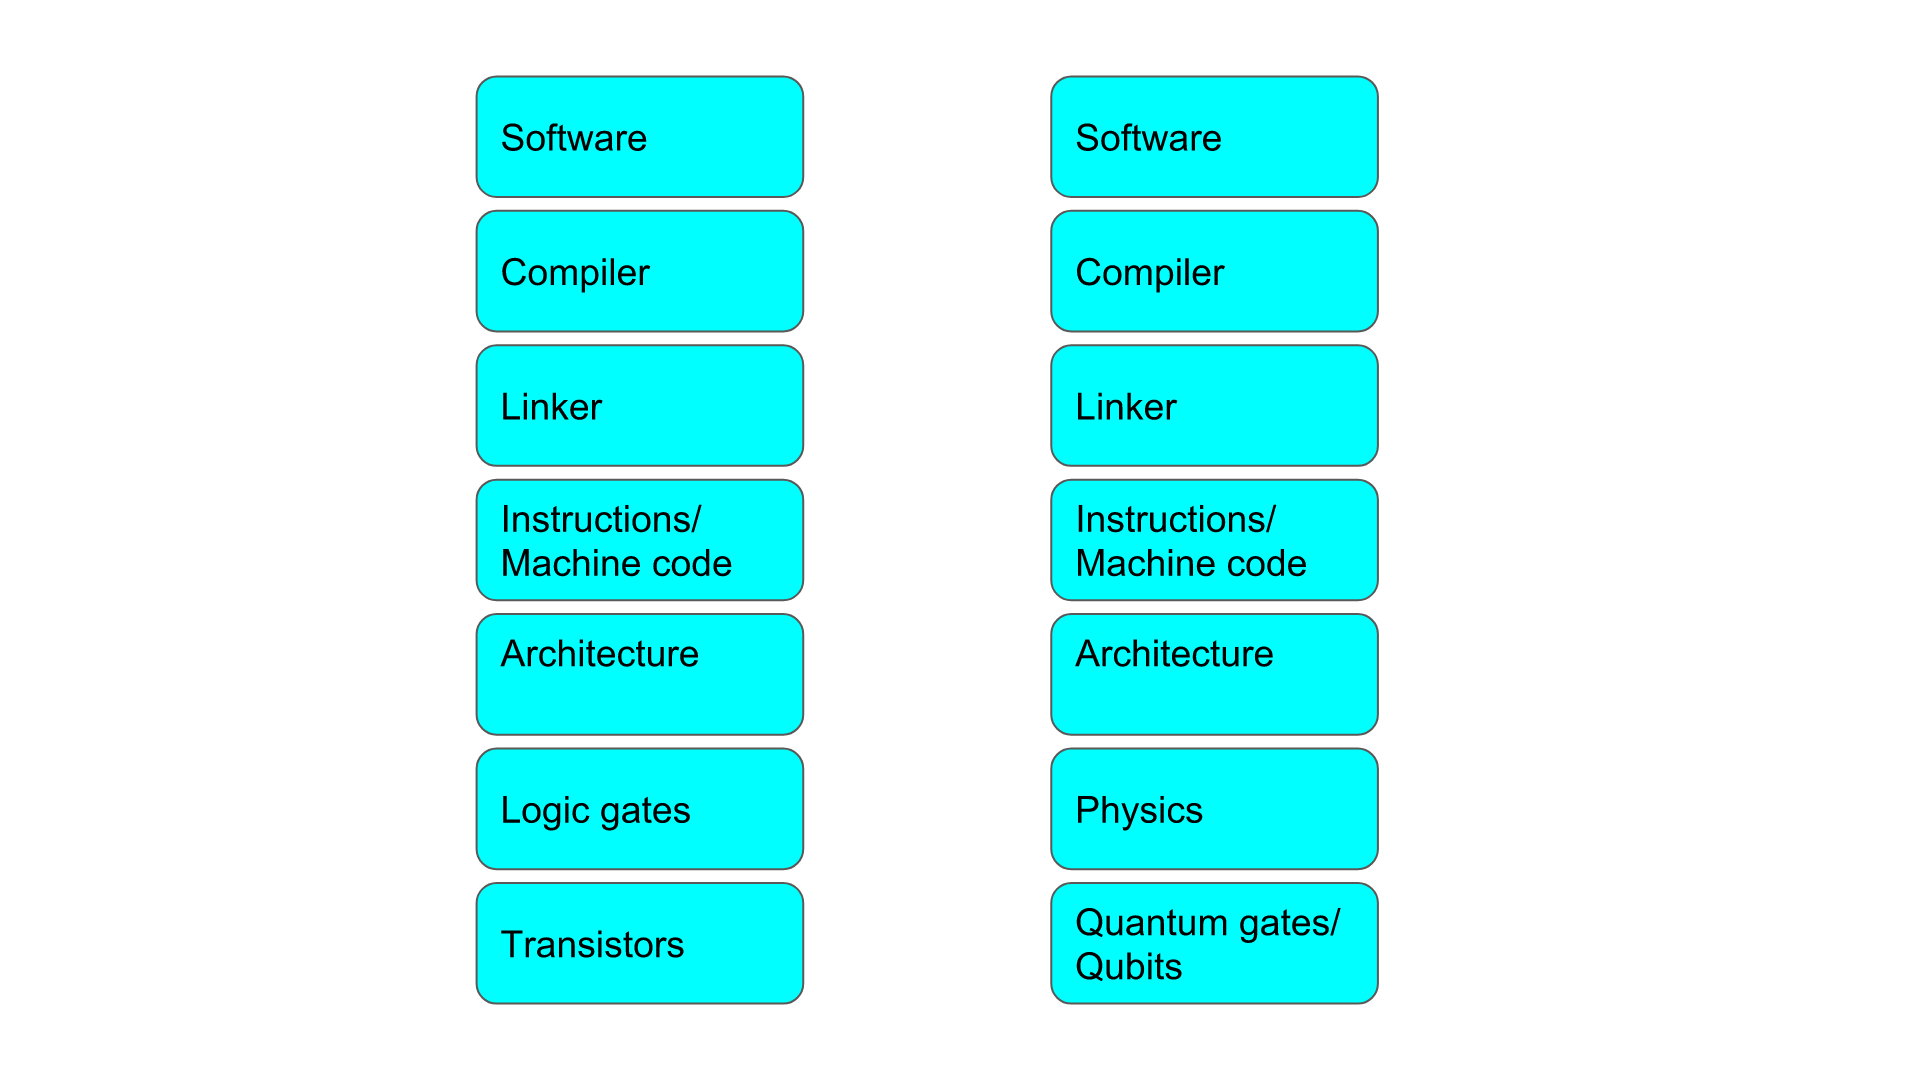
\includegraphics[width=\textwidth]{figures/impl/cpuqpu.png}
    \caption{Caption}
    \label{fig:my_label}
\end{figure}

%abstraction oop or functional
Other levels of abstraction have subsequently been introduced into programming. Some relate to code structure (object oriented programming, functional programming, and other paradigms), and others to the portability of the code. For example, Java runs in an environment called a virtual machine. This is a program which runs a file containing Java source code on a particular computer. The critical difference between this and a compiler is that many computers have a Java virtual machine, so that the end user can just run the same program without having to worry about whether there is a compiler present. 

% nisq devices birth of languages
Quantum programming languages may eventually develop in a similar way. However, there are some important differences. For example, quantum programming languages are being developed without there existing a large scale quantum computer to run programs on. This is due to the hindsight afforded by classical programming languages, and the assumption that quantum programming languages will be essentially similar. Their role is currently to understand the structure of quantum algorithms better and to provide a platform for simulating quantum computers, rather than to make programming quantum computers easier. 

% bad to do single qubits quantum computer with structure
Here, we will consider how the implementation of a large scale quantum computer might inform the structure of quantum languages. For example, most quantum programming languages currently emphasise single qubit manipulation. While this works when we only have a few qubits, it clearly becomes unfeasible in a quantum computer with a million qubits. There, it will be necessary to organise qubits into registers, variables and types depending on their role. What should those types be? How should it be informed by the structure of the quantum computer?

% re configurable logic and memory sections
Part of the issue is the current lack of understanding of large scale quantum computer architectures. A typical classical computer CPU architecture is shown in \autoref{fig:cpuHarvArch}. It contains modules for memory, processing and arithmetic, buses for moving data around, and input/output ports to connect to other devices. The computer is controlled by an instruction set, which is read and decoded in the control section. 

Each instruction performs a basic operation such as moving data from external memory into working memory, adding variables together, etc. There are also control instructions for deciding what to do next, for example branches and sub-routine calls. Memory is often organised into registers, which might be 8 bits wide in a small microcontroller, or 64 bits wide in a modern Intel processor. These instructions are the lowest level of processing available to a classical programming language. 
% 
By analogy, it is likely that a quantum computer will have a similar architecture containing an instruction set (ADD, MOV, etc.). We will consider the possible structure of such an instruction set in \autoref{sec:qinstructions}. We will then consider the simplest type of abstraction above quantum assembly language -- the analogue of C (QLang+-!). We will consider the necessity of quantum compilers and linkers, and how they differ from their classical counterparts in (section). 

%%%%%%%%%%%%%%%%%%%%%%%%%%%%%%%%%%%%%%%%%%%%%%%%%
\subsection{Quantum instruction sets}
\label{sec:qinstructions}

An instruction set is a collection of operations designed to meet two competing requirements. The instructions must contain enough operations to allow access to the full functionality of the computer, without exposing implementation details. Further, it must be simple to express a program in terms of the instruction set, so the instructions should be as high level as possible. However, the instruction set should not be overly large or contain complex operations, otherwise it would be difficult to implement in hardware.

Candidate instruction sets could therefore tend towards two opposite extremes. On the one hand, the instruction set could be very large and implement nearly everything a program might want to do: matrix multiplication, Fourier transforms, database operations, etc. Every operation would be optimised in hardware and all possible tasks would be accounted for. This would make programming and compiling very simple and programs would tend to be very efficient. However, the instruction set would be difficult to implement, and inflexible in the face of new applications and tasks.

On the other end of the scale, the instruction set might be the single operation NAND. This would be universal for classical computation, so all programs could be realised. The design of the computer would be very simple, with only one instruction to implement. However, simple programming tasks such as addition would become very difficult, and complicated programs would be nearly impossible to write.

Classical instructions sets sit between these two extremes. They contain general operations such as arithmetic (ADD, MUL, etc.), copy operations (MOV) and control flow (BRANCH, CALL, etc.) and they also contain some lower level details such as bit manipulation. 

In the rest of this section we consider the instructions which might form the basis of a full quantum computer.

%%%%%%%%%%%%%%%%%%%%%%%%%%%%%%%%%%%%%%%%%%%%%%%%%%%%%%

\subsubsection{Qubit manipulation}

Despite the need for full quantum computers to contain operations on registers, it is likely that they would retain single qubit manipulation. In classical computers single bits can be accessed using bit manipulation instructions.  For example, in the Microchip 16-bit dsPIC family of microcontrollers \cite{microchip2008AsmRef}, bits can be set to zero or one using the BCLR and BSET instructions.

\begin{lstlisting}[language=asm, caption={Single bit operations}]
    CLR     w0      ; clear register w0
    CLR     w1      ; clear register w1
    BSET    w0, #2  ; set bit #2 of register w0 to 1
    BTG     w1, #6  ; toggle bit #6 of register w1
    BCLR    w1, #5  ; clear bit #5 of register w1
\end{lstlisting}

This code initialises the two registers w0, w1 to zeroes, puts a one in the second bit of register w0, and a zero in the fifth bit of register w1. The BTG instruction toggles bit six of w2, swapping its value from one to zero or vice versa. It performs the classical NOT operation.

In quantum computers, there are many more possibilities for single qubit operations other than just setting and clearing bits. As mentioned above \textbf{REF}, a quantum computer should be able to perform all single qubit operations, which are indexed by two continuous parameters. The quantum instruction set may implement a small set of commonly used operations, such as $X$, $Y$, and $Z$. Then the assembly language may look like:

\begin{lstlisting}[language=asm, caption={Quantum X and Y operations}]
    CLR     w0      ; Quantum registers should be initialised to zero
    CLR     w1      
    QBTX    w0, #2  ; Perform an X gate on bit #2 or w0
    QBTY    w1, #5  
\end{lstlisting}

which performs an $X$ gate on the second qubit of register w0, and performs the $Y$ gate on the fifth qubit of register w1. However, the quantum computer would also need to implement arbitrary rotations and phase shifts, as follows:  

\begin{lstlisting}[language=asm, caption={Arbitrary single qubit rotations}]
    QBTX    w0, #2, #30 ; Perform a 30 degree X rotation on bit #2 of w0
    QBTY    w1, #5, #45
    QPHA    w1, #0, #45 ; Perform a 45 degree phase shift on qubit #0 of w1
\end{lstlisting}

Now, the code executes a $30\degree$ $X$-rotation on the second qubit of w0, and a $45\degree$ $Y$-rotation on the fifth qubit of w1.

The instruction set would need to contain a few 2-qubit operations, such as CNOT:
\begin{lstlisting}[language=asm,caption={CNOT operations}]
    CNOT    w0, #0, #1  ; Perform a CNOT between qubits #0 
                        ; (control) and #1 (target) of w0
    CNOT    w0, w2      ; Perform CNOT between all qubits of the
                        ; w0 (control) and w2 (target) register 
    CNOT    w0, w2, #1  ; Perform CNOT between qubit 1 of w0 and w2 
\end{lstlisting}
The CNOT operation and single qubit unitaries allow the implementation of any unitary operation on qubits. Therefore it would not be necessary to include any more two- or N- qubit gates. However, they may be included for convenience, or because they are simple to implement on a particular architecture. For example, the SWAP gate (which swaps the computational basis states) could replace the CNOT gate if it were simpler to implement a SWAP operation. 

A generalisation of the SWAP operation is the QMOV operation, which move the state of one quantum register into another: 
\begin{lstlisting}[language=asm,caption={QMOV operations}]
    QMOV    w0, w1      ; Move the quantum state of w0 to w1
    QMOV    0x1111, w1  ; Move the state stored at address 0x1111 to w1
\end{lstlisting}
This operation is more subtle than its classical counterpart. Copying is not allowed in quantum computing, so the operation would have to be realised as a swap, where the states in w0 and w1 are interchanged. Alternatively, the state might be teleported, which is a process involving measurement of register w0. The implementation of the QMOV is unimportant; the key feature is that the state which was in w0 ends up in w1.

This is actually a critical instruction of a full quantum computer. It is likely that the computer will be implemented in such a way that only a small set of register (the working registers $w_0...w_n$) support the full range of quantum operations. Therefore quantum data will need to be copied back and forth between these registers and quantum RAM, which is a large block of quantum registers whose only purpose is to store quantum states. A typical sequence of operations might be as follows:
\begin{lstlisting}[language=asm,caption={Adding }]
    QMOV    0x11FD, w1      ; Move the quantum state at address 0x11FD to w1
    QMOV    0xFFFF, w2      ; Move the quantum state at address 0xFFFF to w2
    CNOT    w1, w2          ; Perform a CNOT operation across all qubits
    QMOV    w1, 0x11FD      ; Move the states back
    QMOV    w1, 0xFFFF      ; Move the states back
\end{lstlisting}

%%%%%%%%%%%%%%%%%%%%%%%%%%%%%%%%%%%%%%%%%%%%%%%%%%%%%%%%
\subsubsection{Coherent classical operations}

Any operation which can be expressed in a classical computer has a quantum version, which we will call the `coherent' operation. A coherent operation is one that can be performed on superpositions of states. For example, addition can be implemented coherently in a quantum computer. Suppose that there are two quantum registers $\ket{a}$ and $\ket{b}$ whose contents can be interpreted as numbers. For example $\ket{0101}$ and $\ket{1001}$ represent the numbers 5 and 9. Then there is a quantum version of addition, which we will denote QADD, whose action on the states above is $$\text{QADD}\big[\ket{0101},\ket{1001}\big]=\ket{1110}.$$ In other words, it produces the state which corresponds to the result of the sum of $5 + 9 = 14$. However, it also acts on superpositions, so that $5 + 9 = 14$ and $6 + 9 = 15$ could be performed simultaneously: $$\text{QADD}\left[\frac{1}{\sqrt{2}}\big(\ket{0101}+\ket{0110}\big),\ket{1010}\right]=\frac{1}{\sqrt{2}}\big(\ket{1110}+\ket{1111}\big).$$ Now, the two possible results 14 $\ket{1110}$ and 15 $\ket{1111}$ exist in superposition in the output.

This type of operation intrinsically acts on a register containing many qubits. Otherwise it is not possible to interpret the register as a number.

The above example, QADD, is not a valid quantum operation. This is because all quantum operations must be realised as unitary operations acting on a fixed number of qubits. In particular, there must be the same number of qubits in the output of QADD as there are in the input. Implementing this process involves a complicated set of tradeoffs to do with qubit allocation and gate optimisation, as we considered in the section hardware architecture above \textbf{section}.

A valid version of QADD may work as follows:
\begin{lstlisting}[language=asm]
    QADD    w0, w1, w2  ; Add the contents of w0 and w1 and place it in w2
                        ; w0 and w1 don't change but are now entangled with w2
\end{lstlisting}
The important fact about this instruction, which makes it different from the classical version ADD, is that all three registers are considered both inputs and outputs at the same time. The QADD instruction is a unitary operations performed on the registers w0, w1 and w2. This means that w0 and w1 become entangled with w2 after the instruction has been performed.

More complicated classical operations can also be implemented coherently. Consider the function $f(x)$ of the variable $x$, which takes a bitstring of length $N$ to one of length $M$.  We want a quantum operation $Qf$ which can performs the same function as $f$, but which also acts on superpositons. For example, if $f(x)=x^2$, then $Qf$ would act as follows on the superposition of $\ket{2} = \ket{0010}$ and $\ket{0}=\ket{0000}$ as follows: $$Qf\left[\frac{1}{\sqrt{2}}\big(\ket{0010}+\ket{0000}\big)\right]=\frac{1}{\sqrt{2}}\big(\ket{0100}+\ket{0000}\big).$$ This corresponds to the fact that $2^2 = 4$ and $0^2 = 0$, and those two computations can be performed in superposition. As in the case of QADD, this operation must be implemented as a unitary operation acting on a fixed number of qubits. One way of achieving this is defining the unitary map $$\ket{x}\ket{y} \xmapsto{Qf}  \ket{x}\ket{f(x) \oplus y},$$ where $\oplus$ is bitwise XOR. Here, $x$ is a register containing the input $N$ bit number, and $y$ is a $n$ bit register. Then setting $y=\ket{0}$ results in the the value $f(x)$ being written into the $y$ register: $$\ket{x}\ket{0} \xmapsto{Qf}  \ket{x}\ket{f(x)}.$$ This operation is often called the bit oracle. 

This form of $Qf$ can also be used to implement a coherent function of two variables $g(r,s)$. Suppose that $r$ and $s$ are $N$ bits long and the output is again $M$ bits long. By concatenating $r$ and $s$, we get a single $2N$ bit long number, which we will call $x$. Then $f$ can be seen as a function of a single variable $x$, which can be implemented using $Qf$ above. 

For example, consider the implementation of QADD for 2-bit input arguments. The classical function is addition, i.e. $g(r,s) = r+s$. Concatenating $r$ and $s$ gives a new variable $x$. The truth table for the output $g$ for different values of $r$ and $s$ is shown in \autoref{tab:2bitaddtruth}.
\begin{table}[!htb]
    \caption{Truth table for 2-bit addition}
    \label{tab:2bitaddtruth}
    \begin{subtable}{.5\linewidth}
      \centering
        \begin{tabular}{|l|l||l|}
        \hline
        \multicolumn{2}{|c||}{$x$} & $f(x)$\\
        \hline
        $r$ & $s$ & $r+s$ \\ \hline
        00       & 00       & 0000       \\ 
        00       & 01       & 0001       \\ 
        00       & 10       & 0010       \\ 
        00       & 11       & 0011       \\
        01       & 00       & 0001       \\ 
        01       & 01       & 0010       \\ 
        01       & 10       & 0011       \\ 
        01       & 11       & 0100       \\
        \hline
    \end{tabular}
    \end{subtable}
    %
    \begin{subtable}{.5\linewidth}
      \centering
        \begin{tabular}{|l|l||l|}
        \hline
        \multicolumn{2}{|c||}{$x$} & $f(x)$\\
        \hline
        $r$ & $s$ & $r+s$ \\ \hline
        10       & 00       & 0010       \\ 
        10       & 01       & 0011       \\ 
        10       & 10       & 0100       \\ 
        10       & 11       & 0101       \\
        11       & 00       & 0011       \\ 
        11       & 01       & 0100       \\ 
        11       & 10       & 0101       \\ 
        11       & 11       & 0110       \\
        \hline
    \end{tabular}
    \end{subtable} 
\end{table}
Here, it is clear that the variables $r$ and $s$ can be concatenated into a single variable $x$, and that the truth table in \autoref{tab:2bitaddtruth} can be interpreted as a function of a single variable $x$ which maps 4-bit numbers to 4-bit numbers. 

Clearly a quantum computer will need enough instructions to implement all coherent operations of interest. One way to achieve this would be to implement an instruction QFUN which implements an arbitrary reconfigurable coherent operation. The truth table of the classical function could be loaded into a dedicated block of registers $f0,...,fn$. 

For example, consider the function $f(x)$ on a 2 bit variable $x$ defined by the truth table in \autoref{tab:1bitadd}. The function $f(x)$ is the classical XOR operation on 2 bits, but could also be interpreted as the 1-bit half adder (addition modulo 2).
\begin{table}[!htb]
    \caption{Truth table for 1 bit addition}
    \label{tab:1bitadd}
      \centering
        \begin{tabular}{|l||l|}
        \hline
        $x$ & $f(x)$ \\ \hline
        00  & 0      \\ 
        01  & 1       \\ 
        10  & 1       \\ 
        11  & 0       \\
        \hline
    \end{tabular}
\end{table}
This function could be loaded an implemented coherently as follows:
\begin{lstlisting}[language=asm]
    ; Set the function f(x)
    MOV     #0, f0    ; Load the truth table for f(x)
    MOV     #1, f1    ; by moving the truth table outcomes
    MOV     #1, f2    ; into the registers f0...f3
    MOV     #0, f3
    ; Perform the coherent operation
    QFUN    w0, w1      ; Here, w0 contains x. The output
                        ; y will be stored in w1.
\end{lstlisting}

This approach suffers from two key drawbacks. The first is its implementation, which may be very difficult. The hardware would need to decide how to implement the coherent operation, which is a non-trivial resource allocation problem. It would likely be quite difficult to come up with general purpose hardware which produces optimised results for all classical functions $f$. The second more serious problem is the lack of extensibility. Here, the size of the function $f$ (i.e. the number of rows in its truth table) is limited by the number of dedicated registers $f0...fn$. This is especially true of truth tables which are sparse, where most of the dedicated registers represent wasted space. 

A better approach would be to devise a minimal set of instruction which could be used to realise all coherent classical operations. For example, suppose that QADD and QMUL were implemented as follows:
\begin{lstlisting}[language=asm]
    MOV     #2, w0      ; 
    MOV     #3, w1   
    QADD    w0, w1, w2  ; Add 2 by 3 and put the result (5) in w2
    QMUL    w0, w1, w3  ; Multiply 2 by 3 and put the result (6) in w3 
    QADD    w2, w3, w4  ; Add the contents of w2 and w3
\end{lstlisting}
These kind of manipulations can be used to build up any polynomial coherent operation. 

An interesting implementation of the quantum adder is presented by Draper \cite{draper2000addition}. The circuit makes use of the Quantum Fourier Transform to turn addition operations into phase operations, and then uses controlled phase gates to implement the operation. This approach avoids using the carry qubits which are involved in implementing addition based on classical models of addition. The same type of approach is extended by Beauregard \cite{beauregard2003ShorImplementation} to obtain the coherent multiplication operation.

% The paper describes a way of implementing a^x mod N using coherent arithmetic. It should be easy to write assembly for the operation below.

%%%%%%%%%%%%%%%%%%%%%%%%%%%%%%%%55 
\subsubsection{Quantum conditionals}

One of the most important operations in classical computing is the if-statement. This is a control flow operation, which checks whether a condition is true and executes one block of code or another accordingly.

The prototypical conditional operation in many instruction sets is the bit test. For example, BTSC (bit-test skip-if-clear) can be used to implement the classical controlled-NOT gate, with the truth table 
\autoref{tab:classCNOT}.
\begin{table}[!htb]
    \caption{Truth table classical CNOT}
    \label{tab:classCNOT}
      \centering
        \begin{tabular}{|l||l|}
        \hline
        $x$ & $f(x)$ \\ \hline
        00  & 0      \\ 
        01  & 1       \\ 
        10  & 1       \\ 
        11  & 0       \\
        \hline
    \end{tabular}
\end{table}
The operation is performed by testing whether the control bit A is one, and if it is toggle bit B (using BTG). If A is zero, the BTSC causes the BTG line to be skipped.
\begin{lstlisting}[language=asm]
    BTSC    w0, #0 ; comment
    BTG     w0, #1
\end{lstlisting}

In quantum instruction sets, there will almost certainly be classical branching operations, which perform quantum operations that are conditioned on the value of classical bits. However, it is conceivable that there are also quantum conditional operations, where the BTSC instruction above might be generalised to depend on a qubit. For example, the QBTSC instruction would execute the next line of code if the test qubit is in the state one, otherwise the next line would be skipped.

What if the test bit is in a superposition of zero and one? Then the outcome of the program should be to leave the quantum computer in a superposition of executing and not executing the next line of code.

For example, the CNOT gate could be implemented as follows:
\begin{lstlisting}[language=asm]
    QBTSC   w0, #0
    QBTG    w0, #1
\end{lstlisting}
Here, the target (qubit 1 of w0) is toggled depending on the value of the control (qubit 0 or w0). If the control is in the state $$\frac{1}{\sqrt{2}}\big(\ket{0}+\ket{1}\big),$$ then the target would be in a superposition of non-toggled and toggled -- exactly the action of the CNOT gate. 

% Add a section about quantum conditional branching
\begin{comment}
Such an operation could be used to implement the coherent operation of exponentiation, $f(x) = a^x$, where $a$ is some fixed integer and $x$ is a quantum register. The algorithm works by repeatedly multiplying $a$ by itself. Each time $a$ is multiplied by itself, the $x$ register is decremented 
\begin{lstlisting}[language=asm,caption={Compute $a^x$ for $a=3$}]
    ; Set w2 as a superposition 
    MOV     #3, w0  ; Copy a=3 into w0
    MOV     #1, w1  ; Start with #1 in w1
    ; Assume w2 contains x 
A:  QRTBC   w2, B       ; Branch to B if w2 is 0
    QMUL    w1, w0, w1  ; Multiply w1 by w0 and store result in w1 
    QDEC    w2          ; Decrememt w2 by 1 (w2 = w2 - 1) 
    BRA     A           ; Branch to A
B:                  ; w2 now contains 3^x
\end{lstlisting}

\url{https://docs.google.com/presentation/d/1SAYwmZ2yAanG0IhbPK4y2j\_JfoOjs\_K9bXPlLtm7Q0w/edit?usp=sharing}

%https://arxiv.org/abs/1311.1074

\end{comment}

%%%%%%%%%%%%%%%%%%%%%%%%%%%%%%%%%%%%%%%%%%%
\subsubsection{Measurement instructions}

One of the most important features of quantum computing is the ability to measure qubits and collapse the state to one of a particular set of outcomes. Measurements can be made in arbitrary bases, but these can always be reduced to measurement in the computational basis by a suitable choice of single qubit unitary operations. 

The following example shows some possible measurement instructions
\begin{lstlisting}[language=asm,caption={Quantum register measurement}]
    QMEAS   w0, cw1     ; Measure quantum register w0, place result in classical register cw1
    QMEAS   w1, #0, cw1 ; Measure qubit 0 of w0, place the result in cw1
\end{lstlisting}

%%%%%%%%%%%%%%%%%%%%%%%%%%%%%%%%%%%%%%%%%5
\subsubsection{Classical operations}

It makes sense for the instruction set of a quantum computer to contain classical operations as well. Many quantum algorithms (e.g. Shor's factoring algorithm, the variational quantum eigensolver), contain both quantum and classical elements, and so it would be benificial to be able to access both types of operation in the same machine using a consistent syntax. 

This entails the encorporation of many instructions which are standard on classical computers: for example, arithmetic (ADD, MUL), control flow (CALL and BRA), bit manipulation, etc. As discussed in the hardware section \textbf{above}, these would be implemented by classical logic in the classical part of the quantum computing architecture. 

In addition to purely classical operations, some instructions could have hybrid quantum/classical dialects. For example, the addition instruction QADD could add two quantum registers or add a quantum register to a classical register:
\begin{lstlisting}[language=asm,caption={Different dialects of QADD}]
    QADD    w0, w1, w2  ; Add quantum registers w0 and w1 and 
                        ; place result in w2
    QADD    cw0, w0, w1 ; Add classical register cw0 to quantum                      
                        ; register w0 and place the result in w1

\end{lstlisting}
This kind of thing, where a single instruction can take many different types of arguments, is standard in classical instruction sets. Behind the scenes, the instructions might be implemented differently depending on their arguments. For example, as described by Beauregard \cite{beauregard2003ShorImplementation}, it is possible to reduce the number of quantum gates required for adding a classical register to a quantum register, compared to the full operation of adding two quantum registers.


%%%%%%%%%%%%%%%%%%%%%%%%%%%%%%%%%%%%%%%%%
\subsubsection{Quantum types}
The most important of these is a quantum type. Classical types typically include things like `double' (for integers), `char' (for letters), `float' (for floating point number), etc. and possible more complex types like point (which contain references to variables). In a quantum computer, there would have to be a types for a quantum registers. For example, `qdouble' might refer to a quantum register whose contents is interpreted as an integer. A `qbitmap' might refer to a register whose contents is not to be interpreted, i.e. all the qubits should be treated independently.

There would probably not be a qubit type in quantum languages for long-term quantum computers. This is because there would presumably be enough resources that a quantum register (say 8 qubits wide) could be used as a single qubit, but ignoring the other seven qubits. This is similar to the lack of a bit type in modern classical programming languages, for the same reason.

%%%%%%%%%%%%%%%%%%%%%%%%%%%%%%%%%%%%%%%%%
\subsubsection{Quantum operations}
There would need to be fundamental quantum operations. The types of quantum operations would be dictated by the quantum type of the variables which are operands. For example, two variables of type qdouble could be coherently added, but it would not make sense to coherently add two variables of type qbitmap.

There would need to be some facility for implementing quantum measurements. There would need to be some variant of a `measure' keyword, which could be made to either measure registers of single qubits. This might depend on type, so that by default qdouble are measured register wide but qbitmaps require an argument specifying which bit to measure.

There is also the possibility of including quantum conditional operations, such as a quantum if statement. Ignoring for the moment the (extreme) difficulty of implementing such a construction, there are several ways the syntax might work. One is to have a standard if statement which automatically becomes as classical or quantum if depending on the type of the argument. Alternatively, there may be two keywords, cif (classical-if) and qif (quantum-if), which make the distinction obvious in the source code.  

%%%%%%%%%%%%%%%%%%%%%%%%%%%%%%%%%%%%%%%%%%
\subsection{Higher level languages}

The purpose of higher level languages is to provide a readable syntax for common language constructions. These can then be translated by a compiler into assembly language for a particular machine. This removes the need for the programmer to understand machine code, and also makes the language portable across platforms with different instruction sets. 

In classical computing, high level programming languages contain control flow statements (if, for, while, etc.), type checking (e.g. whether a register is interpreted as an integer or a character), syntax for defining functions, etc. 

In a quantum programming language, many of these remain. It would still be of interest to perform classical operations such as classical if-statements and classical function calls. However, there would need to be new features to account for the new quantum elements that are accessible to the programmer, as we describe below.

%%%%%%%%%%%% %%%%%%%%%%%%%%%%%%%%%%%%%%%
\subsection{High- and low- level quantum languages}

functional vs object oriented. High level languages is all about adding abstraction: language constructs are not closely related to computer hardware features, but should be easier/more intuitive to use, and should work across different hardware implementations.

Low level languages:more quantumness, harder to use, but more closely related to hardware and consequently not portable. E.g. assembly based on the instruction set architecture, C constructs are based closely on instructions (if, while, do, based on branch instructions. arithmetic, bit manipulation, variable storage and access are all cpu instructions).

%%%%%%%%%%%%%%%%%%%%%%%%%%%%%%%%%%%%%%%%%%%%%%%%%%%%%
\subsection{Examples of different types of languages}

Discuss the languages included in the language section: Q\#, Quil, Quiskit, Scaffold \footnote{C}. 

The majority of currently available quantum languages are (high level languages with object oriented structure such as Python and C\# but are used as low level languages). As discussed in section \textbf{REF} the languages reduce to listing quantum gate instructions, building up the logic circuit for the algorithm by essentially by hand. This can pose problems for algorithms which make use of a quantum oracle which is a unitary $U(f(x))$ which depends on a classical function $f(x)$ as calculating an optimal reversible version of $f(x)$ is hard classically to compute \textbf{REF (p polling)}.

Python is an interpreted and C\# uses JIT compilation, Scaffold resembles the most compiled language present in our discussion. 

The current languages discussed here use individual qubits focusing on the ability to address each qubit individually. We hope that future languages will avoid doing this as it poses problems for many qubit machines.

%%%%%%%%%%%%%%%%%%%%%%%%%%%%%%%%%%%%%%%%%%%%%%%%%%%%%
\subsection{Compilers}

Compilers break down programming language code into the instruction set of the machine. The compiler is more or less important depending on the amount of abstraction in the language. The difficulty of implementing the compiler depends directly on how much abstraction is already contained in the instruction set. By definition, assembly language does not require a compiler because it is already written in terms of machine instructions. At the moment the machine code of all existing quantum information processors is their gate set, meaning that the compiler must perform gate synthesis (see \autoref{physimp} for a more detailed discussion on gate synthesis). 

This is contrary to the implementation of classical computers, whose instruction set is a much higher level than logic gates. We anticipate that large scale quantum computers will eventually have instruction sets that contain many more quantum operations in addition to quantum gates, meaning that the burden on the compiler will be greatly reduced.

review compiler progress with references. Include the `compiler' for pyquil. comment on the range of meanings `quantum compiler' seems to have. Are there any actual compilers? Is the scaffold compiler legit?

language design what about quantum computing as a whole influences the design of the language for future languages. How does the quantumness show up at different levels of abstraction (i.e. gates at the bottom, quantum-if statements a bit of the way up, ..., languages with no explicit references to quantum stuff?)

%%%%%%%%%%%%%%%%%%%%%%%%%%%%%%%%%%%%%%%%%%%%%%%%%%%%
\subsection{Linkers}

Oli's fault not finished.
connectivity, memory allocation (qubit allocation),  

%%%%%%%%%%%%%%%%%%%%%%%%%%%%%%%%%%%%%%%%%%%%%%%%%%%%%
\section{The future}


\subsection{QLANG $+-$ \textsuperscript{TM} the Quantum programming language}

We introduce the QLANG$+-$\textsuperscript{TM} language qubytes\textsuperscript{TM} and quibbles\textsuperscript{TM}. 
